\documentclass[crop, tikz]{standalone}
\usetikzlibrary{patterns, decorations.pathreplacing}

\begin{document}
    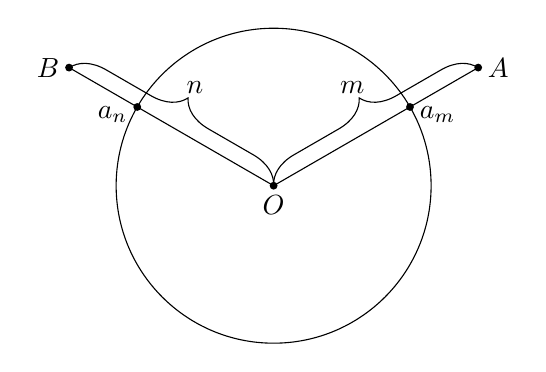
\begin{tikzpicture}
        \coordinate (O) at (0, 0);
        \coordinate (A) at (2.598, 1.5);
        \coordinate (B) at (-2.598, 1.5);
        \coordinate (am) at (1.732, 1);
        \coordinate (an) at (-1.732, 1);

        \draw (O) circle (2);
        \draw (O) -- (A);
        \draw (O) -- (B);

        \draw (O)  node[circle, fill, inner sep=1pt]{} node[below]{$O$};
        \draw (A)  node[circle, fill, inner sep=1pt]{} node[right]{$A$};
        \draw (B)  node[circle, fill, inner sep=1pt]{} node[left]{$B$};
        \draw (am) node[circle, fill, inner sep=1pt]{} node[right, yshift=-0.1cm]{$a_m$};
        \draw (an) node[circle, fill, inner sep=1pt]{} node[left, yshift=-0.1cm]{$a_n$};

        \draw[
            decorate,
            decoration={
                brace,
                amplitude=12pt
            }
        ] (O) -- (A) node[midway, yshift=0.5cm, xshift=-0.3cm]{$m$};

        \draw[
            decorate,
            decoration={
                brace,
                mirror,
                amplitude=12pt
            }
        ] (O) -- (B) node[midway, yshift=0.5cm, xshift=0.3cm]{$n$};
    \end{tikzpicture}
\end{document}
